\begin{figure}[H]
\centering
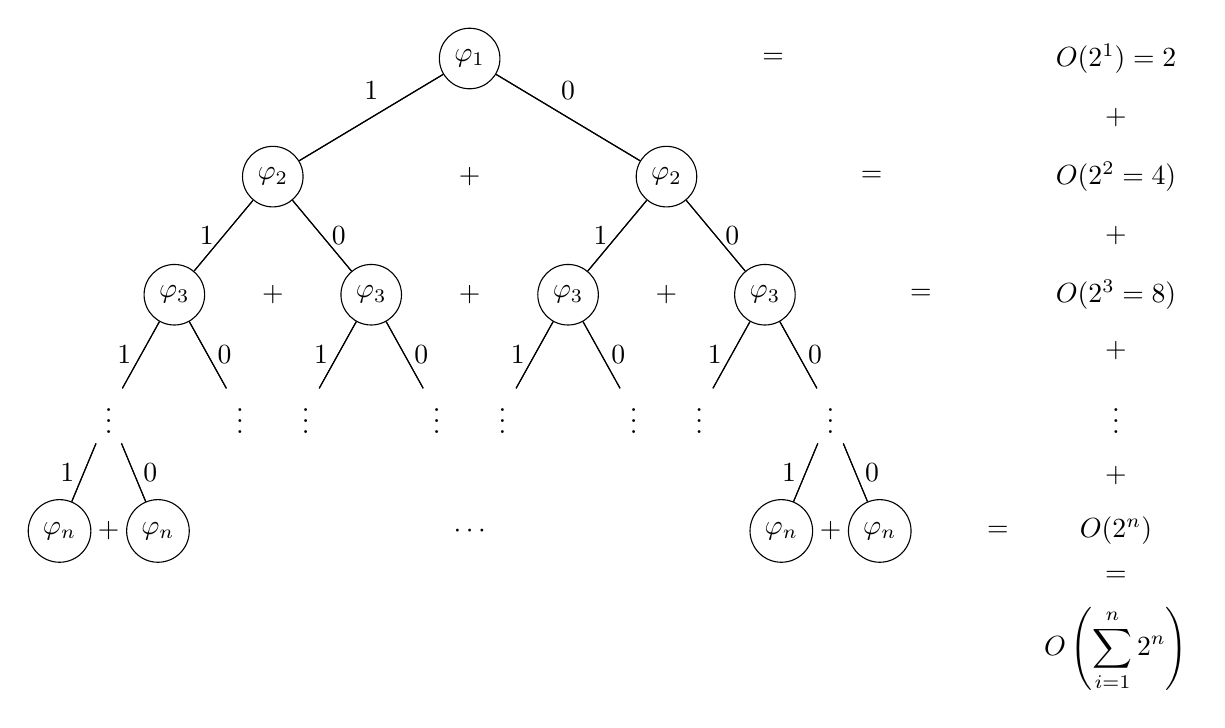
\begin{tikzpicture}[level/.style={sibling distance=50mm/#1}]
\node [circle,draw] (z){$\varphi_{1}$}
  child {node [circle,draw] (a) {$\varphi_{2}$}
    child {node [circle,draw] (b) {$\varphi_{3}$}
      child {node (p1) {$\vdots$}
        child {node [circle,draw] (d) {$\varphi_{n}$}}
        child {node [circle,draw] (e) {$\varphi_{n}$}}
      }
      child {node (p2) {$\vdots$}}
    }
    child {node [circle,draw] (g) {$\varphi_{3}$}
      child {node (p3) {$\vdots$}}
      child {node (p4) {$\vdots$}}
    }
  }
  child {node [circle,draw] (j) {$\varphi_{2}$}
    child {node [circle,draw] (k) {$\varphi_{3}$}
      child {node (p5) {$\vdots$}}
      child {node (p6) {$\vdots$}}
    }
  child {node [circle,draw] (l) {$\varphi_{3}$}
    child {node (p7) {$\vdots$}}
    child {node (c){$\vdots$}
      child {node [circle,draw] (o) {$\varphi_{n}$}}
      child {node [circle,draw] (p) {$\varphi_{n}$}
        child [grow=right] {node (q) {$=$} edge from parent[draw=none]
          child [grow=right] {node (q) {$O(2^{n})$} edge from parent[draw=none]
            child [grow=up] {node (r) {$\vdots$} edge from parent[draw=none]
              child [grow=up] {node (s) {$O(2^{3}=8)$} edge from parent[draw=none]
                child [grow=up] {node (t) {$O(2^{2}=4)$} edge from parent[draw=none]
                  child [grow=up] {node (u) {$O(2^{1})=2$} edge from parent[draw=none]}
                }
              }
            }
            child [grow=down] {node (v) {$O\left(\displaystyle\sum_{i = 1}^n 2^n \right)$}edge from parent[draw=none]}
          }
        }
      }
    }
  }
};
\path (a) -- (j) node [midway] {+};
\path (b) -- (g) node [midway] {+};
\path (k) -- (l) node [midway] {+};
\path (k) -- (g) node [midway] {+};
\path (d) -- (e) node [midway] {+};
\path (o) -- (p) node [midway] {+};
\path (o) -- (e) node (x) [midway] {$\cdots$};
\path (q) -- (r) node [midway] {+};
\path (s) -- (r) node [midway] {+};
\path (s) -- (t) node [midway] {+};
\path (s) -- (l) node [midway] {=};
\path (t) -- (u) node [midway] {+};
\path (z) -- (u) node [midway] {=};
\path (j) -- (t) node [midway] {=};
\path (q) -- (v) node [midway] {=};



\path (z) edge node[above=3pt]{$1$} (a);
\path (z) edge node[above=3pt]{$0$} (j);

\path (a) edge node[left]{$1$} (b);
\path (a) edge node[right]{$0$} (g);
\path (j) edge node[left]{$1$} (k);
\path (j) edge node[right]{$0$} (l);

\path (b) edge node[left]{$1$} (p1);
\path (b) edge node[right]{$0$} (p2);
\path (g) edge node[left]{$1$} (p3);
\path (g) edge node[right]{$0$} (p4);
\path (k) edge node[left]{$1$} (p5);
\path (k) edge node[right]{$0$} (p6);
\path (l) edge node[left]{$1$} (p7);
\path (l) edge node[right]{$0$} (c);

\path (p1) edge node[left]{$1$} (d);
\path (p1) edge node[right]{$0$} (e);
\path (c) edge node[left]{$1$} (o);
\path (c) edge node[right]{$0$} (p);

\end{tikzpicture}
\caption{Posibles valores de verdad por cada variable en un árbol binario.} \label{fig:a3sat02}
\end{figure}